\subsection*{Problema 02}

\textbf{Enunciado:} Calcular la integral:
\begin{align*}
I = \int \dfrac{\sin x \, dx}{1 + \sin x}
\end{align*}

\textbf{Solución:} Para resolver esta integral, aplicamos un truco algebraico sumando y restando $1$ en el numerador. De esta manera, podemos separar la fracción original en dos partes más sencillas de integrar:

\begin{align*}
I &= \int \dfrac{\sin x + 1 - 1}{1 + \sin x} \, dx \\
I &= \int \left( \dfrac{1 + \sin x}{1 + \sin x} - \dfrac{1}{1 + \sin x} \right) dx \\
I &= \int \left( 1 - \dfrac{1}{1 + \sin x} \right) dx
\end{align*}

Aplicando la linealidad de la integración, dividimos el problema en dos integrales independientes:

\begin{align*}
I &= \int 1 \, dx - \int \dfrac{dx}{1 + \sin x} \\
I &= x - \int \dfrac{dx}{1 + \sin x}
\end{align*}

Para resolver la segunda integral, multiplicamos el numerador y el denominador por el conjugado del denominador, es decir, $(1 - \sin x)$:

\begin{align*}
\int \dfrac{dx}{1 + \sin x} &= \int \dfrac{1 - \sin x}{(1 + \sin x)(1 - \sin x)} \, dx \\
&= \int \dfrac{1 - \sin x}{1 - \sin^2 x} \, dx
\end{align*}

Utilizamos la identidad trigonométrica fundamental $\cos^2 x + \sin^2 x = 1$, por lo que $1 - \sin^2 x = \cos^2 x$:

\begin{align*}
\int \dfrac{1 - \sin x}{\cos^2 x} \, dx &= \int \left( \dfrac{1}{\cos^2 x} - \dfrac{\sin x}{\cos^2 x} \right) dx \\
&= \int \left( \sec^2 x - \sec x \tan x \right) dx
\end{align*}

Las integrales inmediatas resultantes son $\sec^2 x$ y $\sec x \tan x$:

\begin{align*}
\int \left( \sec^2 x - \sec x \tan x \right) dx = \tan x - \sec x
\end{align*}

Sustituyendo este resultado de regreso en nuestra expresión principal para $I$, y considerando la constante de integración $C$:

\begin{align*}
I &= x - (\tan x - \sec x) + C \\
I &= x - \tan x + \sec x + C
\end{align*}

Por lo tanto, la solución general de la integral es:
\begin{align*}
\int \dfrac{\sin x \, dx}{1 + \sin x} = x - \tan x + \sec x + C
\end{align*}

\begin{figure}[H]
	\centering
	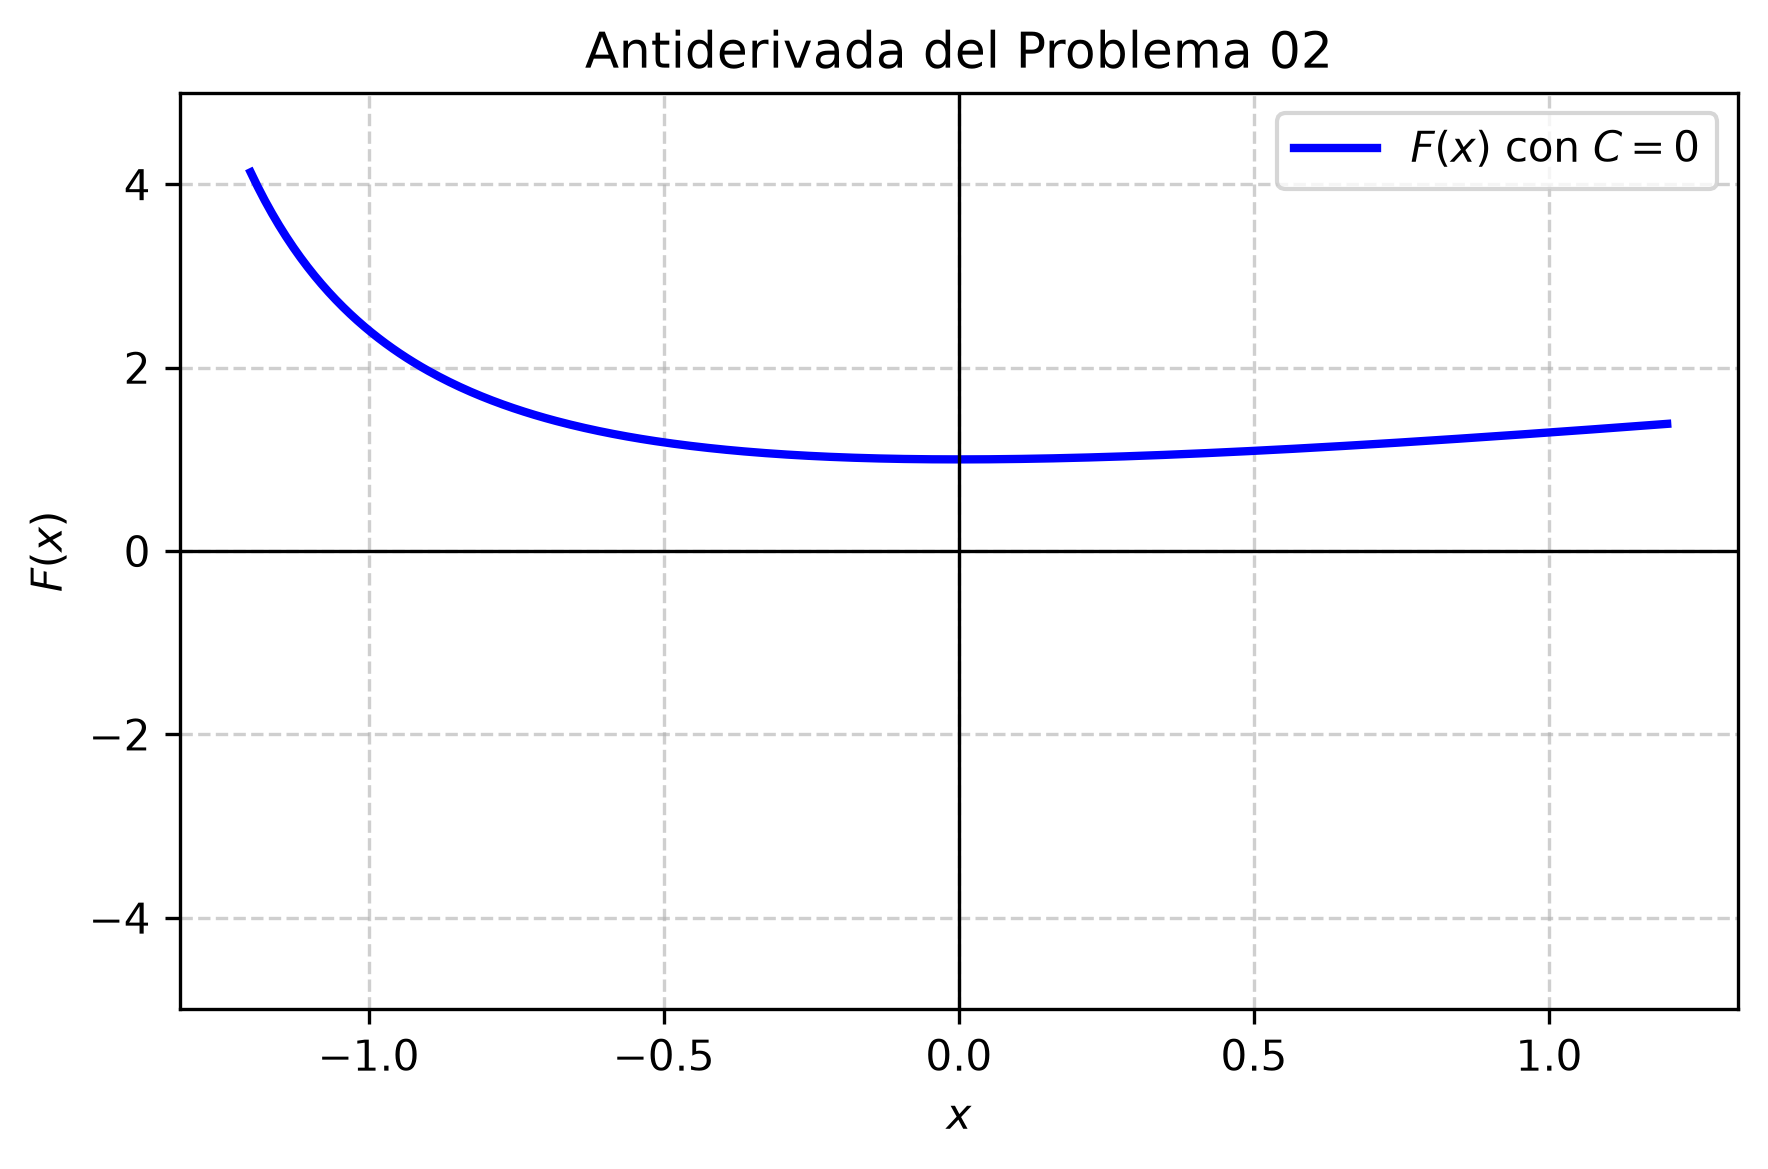
\includegraphics[width=\columnwidth]{semana_04/graficas/SEM04_P02_grafica.png}
	\caption{Representación gráfica de $f(x)$ y su antiderivada $F(x)$ evaluada para la constante de integración $C = 0$ (Problema 02).}
	\label{fig:problema02}
\end{figure}
